% !TEX encoding = UTF-8
% !TEX TS-program = pdflatex
% !TEX root = ../thesis.tex

%************************************************
\chapter{Hadronic Higgs Production}\label{chap:three}
%************************************************

\section{Motivation (better title needed!)}
Here I list various application for the Higgs production cross section and explain why precise predictions are so central. Maybe just put this in the chapter description?
\section{The Leading-Order Cross Section}
Having established, that the gluon-fusion Higgs production cross section is central for many phenomenological applications, we now want to perform the actual \acs{LO} calculation, which was first demonstrated by Georgi et al.\ in 1978~\cite{Georgi:1977gs}. The calculation not only serves as an instructive example on cross section calculation, and thereby allows us to put our experience from section~\ref{sec:2:cross_sections} to good use, but it already introduces many important concepts we can transfer to the \acs{NNLO} computation.

At LO, there are only two possible Feynman diagrams we can draw. They are depicted in Fig.~\ref{fig:4:LO}.
\begin{figure}[h]
\centering
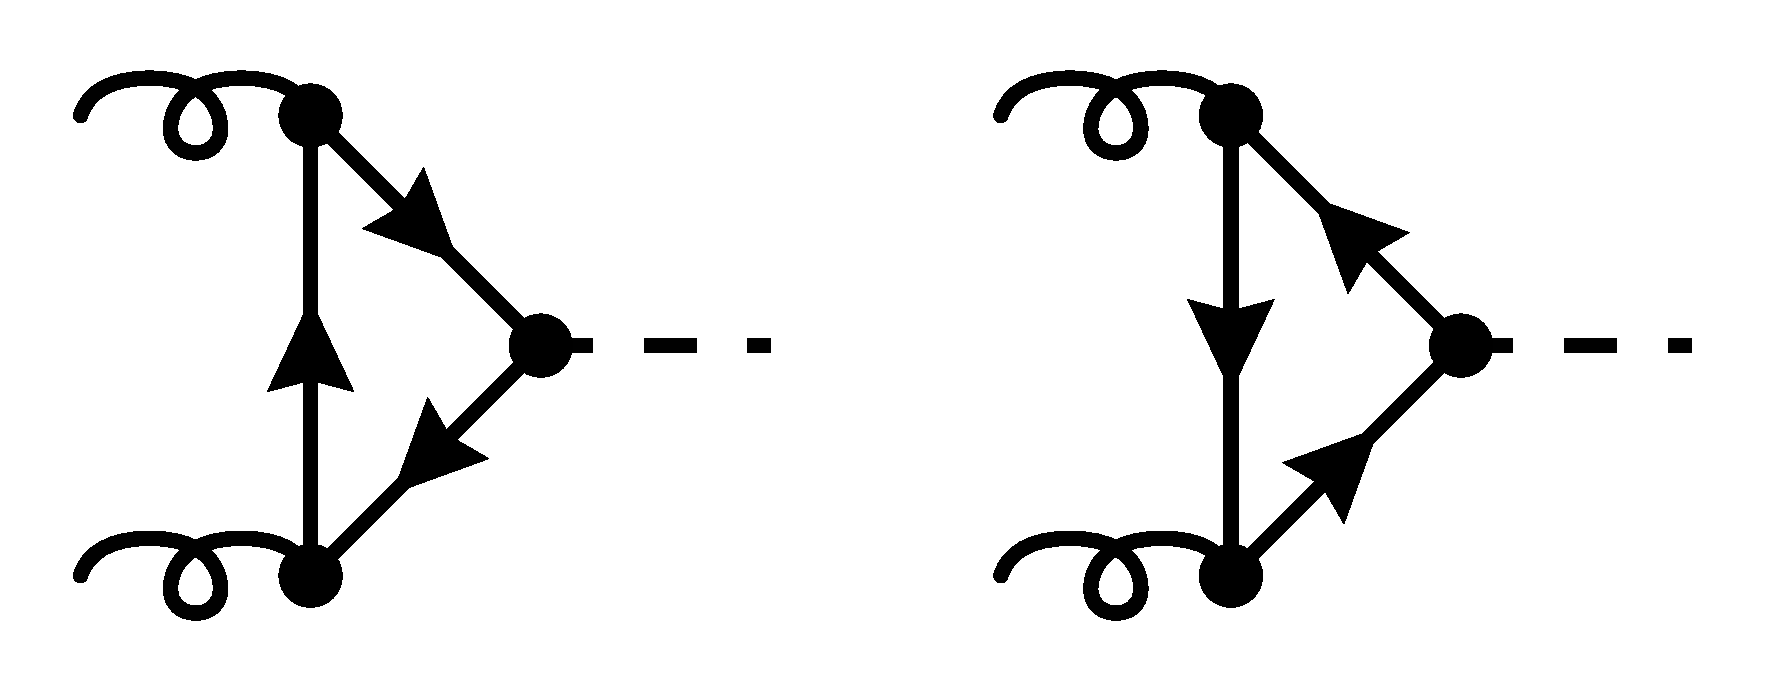
\includegraphics[scale=0.2]{Images/LO.pdf}
\caption{\acs{LO} Feynman diagrams for Higgs production in the gluon-fusion channel.}
\label{fig:4:LO}
\end{figure}
As we can see. Gluon-fusion is a loop induced process with two scales: the mass of the quark running in the loop $m_q$, and the Higgs mass $m_H$ which must simultaneously be the partonic center of mass energy. The initial state gluons carry on the on-shell momenta $p_1$ and $p_2$. Let us then define
\begin{equation}
i\mathcal{M} = i \mathcal{M}^{\mu\nu, ab} \varepsilon_\mu^a(p_1) \varepsilon_\nu^b(p_2).
\end{equation}
With the Feynman rules presented in appendix~\ref{app:1} we find
\begin{equation}
\begin{split}
&i \mathcal{M}^{\mu \nu, ab} = -\int \frac{\dd^4 k}{(2\pi)^4}\, \\
&\quad \times \text{Tr}\!\left[ \frac{-i m_q}{v} \delta_{ij} \frac{i(\slashed{k} + \slashed{p}_1 + \slashed{p}_2 + m_q)}{(k + p_1 + p_2)^2 - m_q^2} (ig \gamma^\nu T^a_{ik}) \frac{i (\slashed{k} + \slashed{p}_1 + m_q)}{(k + p_1)^2 - m_q^2} (i g \gamma^\mu T^b_{kj}) \frac{i (\slashed{k} + m_q)}{k^2 - m_q^2} \right] \\
&\quad + \lbrace p_1 \longleftrightarrow p_2,  \mu \longleftrightarrow \nu, a \longleftrightarrow b \rbrace ,
\label{eq:4:form_factor_amplitude}
\end{split}
\end{equation}
where the extra minus sign in front stems from the fermion trace.

Even without performing the explicit calculation can we already anticipate the general structure of the amplitude. Color wise, the amplitude must be proportional to $\delta^{ab}$, because it is the only available rank-two tensor. Since it is symmetric, the Lorentz structure must also be symmetric in order to satisfy \textit{Bose symmetry}. The only building blocks we have available are $g^{\mu\nu}$, $(p_1^\mu p_2^\nu + p_2^\mu p_1^\nu)$, $p_1^\mu p_1^\nu$, and $p_2^\mu p_2^\nu$, but since all transverse parts drop out of the physical amplitude, the relevant tensors are only $g^{\mu \nu}$ and $p_2^\mu p_1^\nu$. Lastly, we know that the amplitude must satisfy the \textit{Ward identity}, which allows us to restrict the tensor even further, such that we end up with
\begin{equation}
i \mathcal{M}^{\mu \nu, ab} = i\frac{\alphas}{\pi} \frac{1}{v} \delta^{ab} \left(p_2^\mu p_1^\nu - (p_1 \cdot p_2)g^{\mu\nu} \right) \mathcal{C}(m_H, m_q).
\label{eq:4:form_factor}
\end{equation}
Notice that we have only made use of very general properties of the amplitude. This is why the decomposition in Eq.~\eqref{eq:4:form_factor} will hold at every order of $\alphas$. The function $\mathcal{C}(m_H, m_q)$ is called the \textit{Higgs-gluon form factor}. It has mass dimension 0, \ie\ its functional dependence on $m_q$ and $m_H$ must be through a mass ratio
\begin{equation}
\mathcal{C} (m_H, m_q) = \mathcal{C}(z), \quad \text{with} \quad z \equiv \frac{m_H^2}{4 m_q^2}.
\end{equation}
The factor of $1/4$ was introduced, so that the \textit{normal threshold} is located at $z = 1$. Mathematically, this means that $z = 1$ is a solution of the \textit{Landau equations}. Physically, we can interpret the singularity as the point where we have enough energy to produce the quark pair on-shell. We can now project onto the form factor with
\begin{equation}
\mathcal{C}(z) = \frac{\pi v}{i \alphas} \frac{1}{N_c^2 - 1} \delta^{ab} \frac{1}{(p_1 \cdot p_2)^2 (d - 2)} \left(p_{2\,\mu} p_{1\,\nu} - (p_1 \cdot p_2) g_{\mu\nu} \right) i \mathcal{M}^{\mu \nu, ab}.
\end{equation}
Let us define the pertubative expansion of the Higgs-gluon form factor as
\begin{equation}
\mathcal{C} = \mathcal{C}^{(0)} + \frac{\alphas}{\pi} \mathcal{C}^{(1)} + \left( \frac{\alphas}{\pi} \right) \mathcal{C}^{(2)} + \cdots
\label{eq:4:form_factor_expansion}
\end{equation}

If we now insert the \acs{LO} expression of Eq.~\eqref{eq:4:form_factor_amplitude} and perform some basic manipulations we find for the leading coefficient
\begin{equation}
\begin{split}
\mathcal{C}^{(0)} (z) = T_F \frac{1}{2 - 2 \epsilon} \frac{1}{z} \int \frac{\dd^d k}{i \pi^{d/2}} \,&\frac{1}{[k^2 - m_q^2 + i0^+][(k + p_1 + p_2)^2 - m_q^2 + i0^+]} \\
& \times \left( 2 \epsilon + \frac{m_H^2}{[(k + p_1)^2 - m_q^2 + i0^+]} \left(\frac{1}{z} + \epsilon - 1 \right) \right),
\label{eq:4:C0_integral_form}
\end{split}
\end{equation}
which, after inserting integrals and expanding in $\epsilon$, finally reduces to
\begin{equation}
\mathcal{C}^{(0)}(z) = T_F \frac{1}{z} \bigg \lbrace 1 - \left(1 - \frac{1}{z} \right) \left[ \frac{1}{2} \ln\! \left( \frac{\sqrt{1 - 1/z} - 1}{\sqrt{1 - 1/z} + 1} \right) \right]^2 \bigg \rbrace.
\end{equation}
We see that the Higgs-gluon form factor is roughly proportional to the square of the mass of the quark running in the loop. One power of $m_q$ is hereby picked up from the Yukawa coupling. The other factor $m_q$ is a consequence of the scalar coupling to Higgs. Indeed, without the quark mass, the trace in Eq.~\eqref{eq:4:form_factor_amplitude} would contain an odd number of gamma matrices and vanish consequently. Physically, we can interpret this as a helicity flip of the internal quark at the Higgs interaction vertex. And since massless \acs{QCD} conserves helicity, the other helicity flip is provided by the mass. Similarly, since the two incoming gluons are vector bosons which should form a spinless final state, we would expect them to always carry opposite spins. This intuition is indeed confirmed by the tensor structure of the amplitude \eqref{eq:4:form_factor}, as it always vanishes once contracted with two polarization vectors of the same helicity\footnote{This can be seen easily by boosting to the center of mass frame and using $\epsilon^\mu (-\mathbf{p}, \lambda) \propto \epsilon^\mu (\mathbf{p}, -\lambda)$.}.

The \acs{LO} Higgs-gluon form factor is plotted in Fig.~\ref{fig:4:form_factor}.
\begin{figure}[h]
\centering
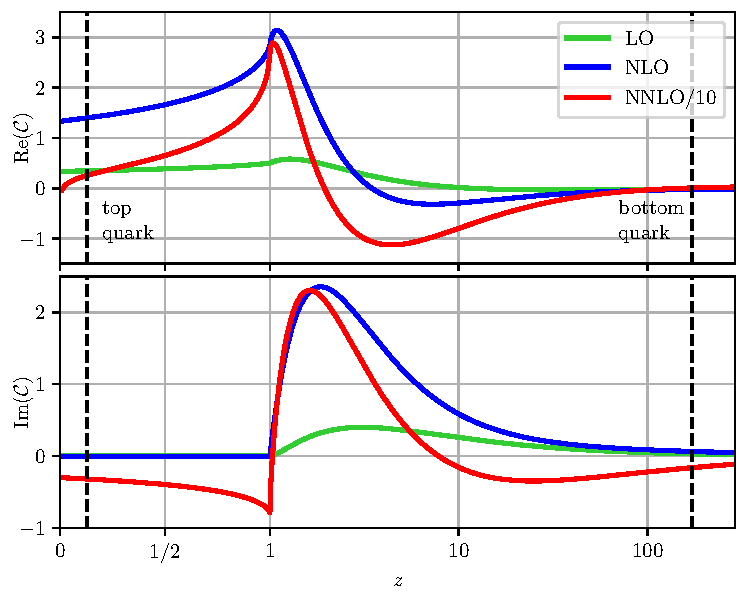
\includegraphics[width=\figurewidth]{Images/form_factor.pdf}
\caption{Real and imaginary part of the finite part of the Higgs-gluon form factor at various perturbative. \acs{NNLO} is divided by ten for better visibility. \acs{NNLO} results also depend on the number of light quark flavors, which has been set to 5 (5\acs{FS}). Top-quark is renormalized in the \acs{OS} scheme. Infrared divergences are subtracted in the \MS\ scheme with the help of the $\mathbf{Z}$ operator (see \eg\ Ref.~\cite{Czakon:2014oma}). Vertical lines indicate the $z$ values for the top and bottom quark masses. The plot was created using the results of Ref.~\cite{Czakon:2020vql}.}
\label{fig:4:form_factor}
\end{figure}
As expected, we pick up an imaginary part starting from the normal threshold at $z=1$. If we expand the form factor around large quark masses, \ie\ we perform a \textit{large mass expansion} (\acs{LME}), we find that it approaches a constant
\begin{equation}
\mathcal{C}^{(0)}(z) = T_F \left( \frac{2}{3} + \frac{7}{45} z + \frac{4}{63} z^2 + \BigO{z^3} \right).
\label{eq:4:LME}
\end{equation}
We will discuss the infinite mass limit in more detail in section~\ref{sec:4:HTL}. On the other side of the spectrum we can see that if the mass of the Higgs is far greater than the mass the internal quark, the form factor is approximately
\begin{equation}
\mathcal{C}^{(0)}(z) = \frac{T_F}{4z} \left[ 4 - \log^2\!\left(-4 z \right) + \frac{1}{z} \left( \log\!\left(-4 z \right) + \log^2\!\left(-4 z \right) \right) + \BigO{1/z^2} \right].
\end{equation}
This expansion is known as \textit{high-energy limit} \acs{HEL}. The appearing double logarithms $\log^2 (m_q^2/m_H^2)$ originate from a soft quark exchange. In fact, the quark mass acts as an infrared regulator of the integral in Eq.~\ref{eq:4:C0_integral_form}, so the appearance of these logarithms is not entirely unexpected. Numerically, these logarithms can be very large. The bottom quark, for example will yield a double logarithm of about $46$. \Ie, although suppressed by a factor of $m_q^2/m_H^2$, the contributions from lighter quark flavors are logarithmically enhanced and hence highly significant for precision predictions.

If we now apply Eq.~\eqref{eq:2:Xsec} and perform the phase space integration, which for a single particle is trivial because of the momentum conserving delta function, we get for the partonic cross section
\begin{equation}
\hat{\sigma}_{gg \rightarrow H}(\tau S) = \frac{\pi}{64 v^2} m_H^2 \left( \frac{\alphas}{\pi} \right)^2 |\mathcal{C}(z)|^2 \delta\! \left(\tau S - m_H^2 \right) \frac{1}{1 - \epsilon}.
\label{eq:4:ggH_cross_section}
\end{equation}
The initial state was averaged over spin and color. In conventional dimensional regularization, the gluons have $d - 2 = 2 (1 - \epsilon)$ spin degrees. Finally, after the convolution with the partonic luminosity we arrive at the LO cross section
\begin{equation}
\sigma_{ggH}^{\text{LO}}(S) = \frac{\pi}{64v^2} \left(\frac{\alphas}{\pi} \right)^2 \mathcal{L}_{gg}\!\left(\frac{m_H^2}{S} \right) |\mathcal{C}^{(0)}(z)|^2.
\end{equation}
From Fig.~\ref{fig:4:form_factor} we can see that the top quark exerts the largest impact on the Higgs-gluon form factor and hence the \acs{LO} hadron cross section. We can read off the partonic luminosity from Fig.~\ref{fig:2:luminosity} and find that the cross section for the top quark induces Higgs production reads\footnote{Values of masses and coupling constants are provided in the \hyperref[chap:notation_and_conventions]{conventions}.}
\begin{equation}
\sigma_{ggH}^{\text{LO}} (t) = 16.30\ \GeV
\end{equation}
at a hadronic center of mass energy of $13\ \text{TeV}$. Although expected to have little impact, we can also include the effects of finite bottom quark masses by coherently summing together the corresponding form factors. We find
\begin{equation}
\sigma_{ggH}^{\text{LO}}(t+b) = 14.72\ \GeV,
\end{equation}
\ie\ the bottom quark lowers the cross section by around $9\%$ at \acs{LO}.

Without the inclusion of electro-weak corrections, we can always decompose the gluon fusion cross section in terms of the Yukawa couplings $Y_i$:
\begin{equation}
\sigma_{ggH} =  \sum_{i\le j} Y_i Y_j \sigma_{i j}.
\end{equation}
We call
\begin{equation}
\sigma_{i \times j} = Y_i Y_j \sigma_{ij},
\end{equation}
the \textit{i-j-interference contribution} and
\begin{equation}
\sigma_{i} = Y_i^2 \sigma_{ii}
\end{equation}
the \textit{pure-i contribution} to the cross section. Both contributions are depicted at \acs{LO} in Fig.~\ref{fig:4:quark_effects}.
\begin{figure}[h]
\centering
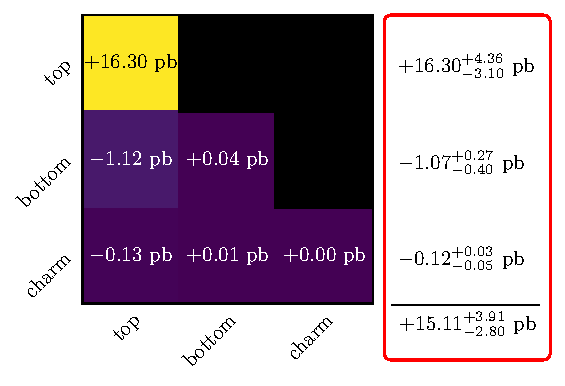
\includegraphics[scale=0.9]{Images/quark_effects_LO.pdf}
\caption{$\sigma_{i}$ (diagonals) and $\sigma_{i \times j}$ (off-diagonals) at \acs{LO} for the three heaviest quark flavors. The red box indicates the sum of each row, and hence the combined effects of each additional flavor. The computational setup is described in the \hyperref[chap:notation_and_conventions]{conventions}.}
\label{fig:4:quark_effects}
\end{figure}
Clearly, the dominant contribution for the lighter quark flavors comes from the interference with the top-quark. The pure-bottom contribution is already below a percent and the pure-charm quark mass effects are completely negligible. The inclusion of the charm quark lowers the total cross section by around $2\%$, making it relevant for high precision predictions.


\section{The Heavy-Top Limit} \label{sec:4:HTL}
The computation of the Higgs production cross section in full \acs{QCD} is quite challenging. As we saw above, even at leading order we encounter loop integrals with two mass scales. It is therefore maybe not surprising that the first \acs{NLO} corrections to this process were actually computed in an approximation framework~\cite{Dawson:1990zj}. In the approximation, we assume that the quark, which is coupling to the Higgs is infinitely heavy. That means we are only interested in the leading term of the \acs{LME}.

The finite distance interaction of the gluon and the Higgs will therefore shrink down to a point like vertex, which we can describe with the effective Lagrangian
\begin{equation}
\mathcal{L}_{\text{HTL}}^{(0)} = \mathcal{L}_{\text{QCD}}^{(n_f - 1)} - C_1 \frac{H}{v} \frac{1}{4} G^a_{\mu \nu} G^{a\, \mu\nu}.
\label{eq:4:HTL_lagrangian}
\end{equation}
We see that the coupling constant now has mass dimension $-1$, so the theory will not be \acs{UV} renormalizable. That means that we cannot absorb all \acs{UV} divergences into multiplicative renormalization constants as we did for the \acs{SM} (see Eq.~\eqref{eq:2:renormalization}), but we will generate more and more independent terms in our Lagrangian to cancel all appearing divergences. On the other hand, as long as we restrict ourselves to \acs{QCD} corrections, and hence only single operator insertions, we can treat the color singlet Higgs as a constant, and renormalize only the gauge invariant operator
\begin{equation}
\mathcal{O}_1 \equiv - 1/4 G_{\mu\nu}^a G^{a\, \mu\nu}.
\end{equation}
To indicate the pertubative order we gave the Lagrangian in Eq.~\eqref{eq:4:HTL_lagrangian} a superscript. The superscript $n_f - 1$ of the QCD Lagrangian specifies the number of active flavors. It was reduced by one, since the heaviest quark flavor was integrated out. The constant $C_1$ is called a \textit{Wilson coefficient}, and it needs to be matched to the full theory in the infinite quark mass limit. At \acs{LO} for example, we find that the Higgs-gluon form factor in the effective theory simply reads
\begin{equation}
C_1 = - \frac{\alphas}{\pi} \mathcal{C}^{(0)} + \BigO{\alphas^2}.
\end{equation}
If we compare this to the leading term of our \acs{LME}~\eqref{eq:4:LME}, we find
\begin{equation}
C_1 = -\frac{\alphas}{\pi} \frac{2}{3} T_F + \BigO{\alphas^2}.
\end{equation}

The main benefit of the approximation lies in the reduced complexity. By integrating out the top quark, we have reduced a loop-induced process to a tree-level process. Moreover, the top-quark mass is eliminated as a scale, hence the appearing Feynman integrals will generally be much simpler to solve.

\subsection{Renormalization of Gauge Invariant Operators}
Beyond \acs{LO} gauge invariant operator like $\mathcal{O}_1$ can mix under renormalization with other gauge invariant operators but notably also with operators which are not gauge invariant. In general, we distinguish two types of operators: \textit{Type-II operators}, which give zero when sandwiched between physical states, and \textit{type-I operators}, which can give non-zero matrix elements. The type-II operators can be further subcategorized into operators vanishing by the equation of motion (\textit{type-II${}_a$ operators}), and all other operators (\textit{type-II${}_b$ operators}). For a polynomial operator with ghost number zero satisfying
\begin{equation}
s \mathcal{O} = 0,
\end{equation}
where $s$ is the \textit{linearized Slavnov operator}, one can proof~\cite{Kluberg-Stern:1974iel, Joglekar:1975nu, Henneaux:2011rma} that
\begin{equation}
\mathcal{O} = s F + \text{gauge invariant operators}.
\end{equation}
Operators of the form $s F$ are also called \textit{Bechi-Rouet-Stora-Tyutin-} (BRST-) \textit{exact operators}, and they vanish between physical states. For $\mathcal{O}_1$ the above conditions are met, allowing us to conclude that the $\mathcal{O}_{II}$ operators are BRST-exact. This can be leveraged to find the complete operator basis:
\begin{equation}
\begin{split}
\mathcal{O}_{I} &\begin{cases} &\mathcal{O}_1 = -\frac{1}{4} G^a_{\mu \nu} G^{a\, \mu\nu}, \\
&\mathcal{O}_2 = \sum_{i=1}^{n_l} m_i \bar{q}_i q_i, \end{cases} \\
\mathcal{O}_{II_a} &\begin{cases} &\mathcal{O}_3 = \sum_{i=1}^{n_l} \bar{q}_i \left( \frac{i}{2} \overleftrightarrow{\slashed{D}} - m \right) q_i, \end{cases} \\
\mathcal{O}_{II_b} &\begin{cases} &\mathcal{O}_4 = A^{a\, \mu} D^\nu G_{\nu\mu}^a + g \sum_{i=1}^{n_l} \bar{q}_i \slashed{A} q_i - \partial^\mu \bar{c}^a \partial_\mu c^a, \\
&\mathcal{O}_5 = D_\mu \partial^\mu \bar{c}^a c^a. \end{cases}
\end{split}
\label{eq:4:operators}
\end{equation}
The operator basis is constructed only of light fields, and the light fields are defined in a decoupled theory.

Since operators of type II cannot generate non-vanishing $S$-matrix elements through renormalization the renormalization matrix must have the general structure
\begin{equation}
\begin{pmatrix}
\mathcal{O}_{I}^R \\
\mathcal{O}_{II}^R
\end{pmatrix} = \begin{pmatrix}
z^{I,I} & z^{I,II} \\
0 & z^{II,II}
\end{pmatrix} \begin{pmatrix}
\mathcal{O}_{I}^B \\
\mathcal{O}_{II}^B
\end{pmatrix}.
\label{eq:4:renormalization_matrix}
\end{equation}
The final form of our effective Lagrangian therefore reads
\begin{equation}
\mathcal{L}_{\text{HTL}} = \mathcal{L}_{\text{QCD}}^{(5)} + \frac{H}{v} \sum_{i=1}^5 C_i^B \mathcal{O}_i^B.
\label{eq:4:lagrangian_operator_basis}
\end{equation}
As usual, we replace the bare quantities by their renormalized counter parts
\begin{equation}
C_i^B \mathcal{O}_i^B = C_i^B  Z_{ij}^{-1} \mathcal{O}_j^R,
\end{equation}
and we identify
\begin{equation}
C^R = (Z^{-1})^T C^B.
\end{equation}
Using the \acs{RGE} we find that the \textit{anomalous dimension} matrix of the Wilson coefficients is determined through
\begin{equation}
\frac{\dd C^R}{\dd \ln \mu} = \left(Z \frac{\dd (Z^{-1})}{\dd \ln \mu} \right)^T  C^R = - \left( \frac{\dd Z}{\dd \ln \mu} Z^{-1} \right)^T \equiv \gamma^T C^R .
\label{eq:4:anomalous_dimension_matrix}
\end{equation}
With the structure of the renormalization matrix~\eqref{eq:4:renormalization_matrix}, we arrive at an important conclusion: The Wilson coefficients of type-II operators cannot mix into the Wilson coefficients of type-I operators through the running in the scale. Since the type-II operators render no contribution to the scattering matrix element, we can focus our attention on the gauge invariant operators and their Wilson coefficients.

We now want to determine the $I,I$ part of the renormalization matrix, \ie\ $z^{I,I}$ to determine the running of the Wilson coefficients. Let us start by defining the generating functional
\begin{equation}
\begin{gathered}
Z[J] \equiv z[J]/z[0], \quad z[J] \equiv \int \prod_i \mathcal{D} \Phi_j\, e^{i(S + J \cdot \Phi)}, \quad S = S[A, c, \bar{c}, q, \bar{q}] \equiv \int \dd^d x\, \mathcal{L}, \\
J = \left( J^\mu, \bar{J}, J, \bar{\eta}, \eta \right), \quad \Phi = \left(\frac{1}{g} A_\mu, c, \bar{c}, q, \bar{q}\right),
\end{gathered}
\end{equation}
with the Lagrangian
\begin{equation}
\mathcal{L} \equiv -\frac{1}{4g^2} F^a_{\mu\nu} F^{a \, \mu \nu} - \frac{1}{2 \xi g^2} \left(\partial \cdot A \right)^2 + \partial^\mu \bar{c}^a D_\mu c^a + \bar{q} \left(\frac{i}{2} \overleftrightarrow{\slashed{D}} - m_q \right) q.
\end{equation}
The Lagrangian is the QCD Lagrangian with only one active quark flavor and rescaled gauge fields
\begin{equation}
A^a_\mu \longrightarrow \frac{1}{g} A^a_\mu.
\end{equation}
The operators in Eq.~\eqref{eq:4:operators} can now be generated by applying the differential operators\footnote{We only provide the operators for the type-I operators, since they are the only ones necessary for computing physical amplitudes. }
\begin{equation}
\begin{split}
&D_1 = - \frac{1}{2}g \frac{\partial}{\partial g} + \xi \frac{\partial}{\partial \xi} - \frac{1}{2} J_\mu \cdot \frac{\delta}{\delta J_\mu}, \\
&D_2 = - m_q \frac{\partial}{\partial m_q}, \\
\end{split}
\label{eq:4:differential_operators}
\end{equation}
on the generating functional
\begin{equation}
z_{\mathcal{O}_k}[J] \equiv \int \prod_j \mathcal{D} \Phi_j \, \hat{\mathcal{O}}_k(0) e^{i(S + J \cdot \Phi)} = - i D_k z[J].
\end{equation}
Here $\hat{\mathcal{O}}_k(0)$ is the Fourier transform of the operator $\mathcal{O}(x)$ at zero momentum. The normalization of the generating functional then properly subtracts the vacuum expectation value of the operators
\begin{equation}
-i D_k Z[J] = \frac{1}{z[0]}\int \prod_j \mathcal{D} \Phi_j \, \left(\hat{\mathcal{O}}_k(0) - \braket{\Omega | \mathcal{O}_k(0) |\Omega} \right) e^{i (S + J \cdot \Phi)} \equiv Z_{\mathcal{O}_k}.
\end{equation}
In the \MS\ scheme, the $R$-operation commutes with the differential operators in Eq.~\eqref{eq:4:differential_operators}, \ie\ the renormalized operators can be generated from the renormalized generating functional
\begin{equation}
Z_{\mathcal{O}_k^R} = -i D_k Z^R[J],
\end{equation}
where the renormalized generating functional is defined as
\begin{equation}
\begin{gathered}
Z^R[J] = z^R[J]/z^R[0] ,\\
\quad z^R[J] = \int \prod_i \mathcal{D}\Phi_j \, e^{i(S^R + J \cdot \Phi)}, \\
S^R \equiv S[Z_3^{\prime\, 1/2} A^R, Z_3^{\prime\, -1/2} c^R, \tilde{Z}_3^{-1/2}\bar{c}^R, Z_2^{1/2} q^R, Z_2^{1/2} \bar{q}^R, Z_g g, Z_m m_q, Z_g^{-2} Z_3^\prime \xi^R].
\end{gathered}
\end{equation}
Using the chain rule we find that
\begin{equation}
-i D_k z^R[J] = \int \prod_j \mathcal{D} \Phi_j \, \left[ \hat{O}_k(0) + \sum_i (D_k \ln Z_i)  \frac{\partial S^R}{\partial \ln Z_i}\right] e^{i S^R + J \cdot \Phi}, \quad Z_i \in \big \lbrace Z_3^\prime , \tilde{Z}_3, Z_2, Z_g, Z_m \big \rbrace.
\end{equation}
And with
\begin{equation}
Z_g \frac{\partial S^R}{\partial Z_g} = - 2 \hat{\mathcal{O}}_1(0), \quad \text{and} \quad Z_m \frac{\partial S^R}{\partial Z_m} = - \hat{\mathcal{O}}_2(0),
\end{equation}
we find that the renormalization constants are given by
\begin{equation}
\begin{alignedat}{2}
&z^{I,I}_{11} = 1 - 2 D_1 \ln Z_g = 1 + g\frac{\partial \ln Z_g}{\partial g}, \quad &&z^{I,I}_{12} = - D_1 \ln Z_m = \frac{g}{2} \frac{\partial \ln Z_m}{\partial g} \\
&z^{I,I}_{21} = 0, \quad &&z^{I,I}_{22} = 1.
\end{alignedat}
\label{eq:4:renormalization_matrix_coefficients}
\end{equation}
Here we made use of the fact, that the \MS-renormalization constants are independent of the quark mass and the gauge parameter. We can rewrite the appearing derivatives in terms of the $\beta$-function and the mass-anomalous dimension. Indeed,
\begin{equation}
\begin{gathered}
\frac{4\pi}{\alphas} \bar{\beta} \equiv \frac{\dd \ln \alphas}{\dd \ln \mu} = - \frac{\dd \ln Z_{\alphas}}{\dd \ln \mu} = - \left( \frac{\partial \ln Z_{\alphas}}{\partial \ln \alphas} \frac{\dd \ln \alphas}{\dd \ln \mu} + \frac{\partial \ln Z_{\alphas}}{\partial \ln\mu} \right) = - \left(  \frac{4 \pi}{\alphas}\bar{\beta} \frac{\partial \ln Z_{\alphas}}{\partial \ln \alphas} + 2 \epsilon \right) \\
\Rightarrow \frac{\partial \ln Z_{\alphas}}{\partial \ln \alphas} = g \frac{\partial \ln Z_g}{\partial g} = - 1 - 2 \epsilon \frac{\alphas}{4 \pi\bar{\beta}} = -1 + \frac{1}{1 - \frac{\beta}{2 \epsilon} \frac{4 \pi}{\alphas}},
\end{gathered}
\end{equation}
where in the last step we used the relation between the $d$- and four-dimensional $\beta$-functions
\begin{equation}
\bar{\beta} = \beta - 2 \epsilon \frac{\alphas}{4 \pi}.
\label{eq:4:d_dimensional_beta_function}
\end{equation}
Similarly, we find
\begin{equation}
\begin{gathered}
\gamma_m \equiv - \frac{\dd \ln m_q}{\dd \ln \mu} = \frac{\dd \ln Z_m}{\dd \ln \mu} = \frac{\partial \ln Z_m}{\partial \ln \alphas} \frac{\partial \ln \alphas}{\partial \ln \mu} = \frac{\partial \ln Z_m}{\partial \ln \alphas} \frac{4 \pi}{\alphas} \bar{\beta} \\
\Rightarrow \frac{\partial \ln Z_m}{ \partial \ln \alphas} = g \frac{\partial \ln Z_m}{\partial g} = \frac{\alphas}{4 \pi} \frac{1}{\bar{\beta}} \gamma_m = - \frac{\gamma_m}{2 \epsilon} \frac{1}{1 - \frac{\beta}{2 \epsilon} \frac{4 \pi}{\alphas}}
\end{gathered}
\end{equation}

Finally, we want to use the above results to calculate the anomalous dimension matrix in Eq.~\eqref{eq:4:anomalous_dimension_matrix}. The entries of the renormalization constant only depend on scale through the coupling constant, \ie\
\begin{equation}
\gamma^{I,I} = -\frac{\dd z^{I,I}}{\dd \ln \mu} (z^{I,I})^{-1} \bigg \vert_{\epsilon = 0} = -\frac{\partial z^{I,I}}{\partial \alphas} (z^{I,I})^{-1} 4 \pi \bar{\beta} \bigg \vert_{\epsilon = 0} = \frac{\partial z^{I,I\,(1)}}{\partial \alphas} 2 \alphas.
\end{equation}
Where we used that $z^{I,I}$ consists only of poles in the \MS\ scheme, and once again applied the relation between the $\beta$-functions in Eq.~\eqref{eq:4:d_dimensional_beta_function}. $z^{I,I\, (1)}$ denotes the residue of the renormalization matrix
\begin{equation}
z^{I,I} = \mathbb{1} + \sum_{i = 1} z^{I,I\,(i)} \epsilon^{-i}.
\end{equation}
We then find for the anomalous dimension matrix
\begin{equation}
\gamma^{I,I} = \begin{pmatrix} 4 \pi \alphas \frac{\dd}{\dd \alphas} \left( \frac{\beta}{\alphas} \right) & - \alphas \frac{\dd \gamma_m}{\dd \alphas} \\
0 & 0 \end{pmatrix}.
\end{equation}
The structure of this matrix reveals, that the $C_1$ Wilson coefficient, which is relevant coefficient for the  \acs{HTL}, is completely independent of the other Wilson coefficients. The \acs{RGE} for the Wilson coefficient~\eqref{eq:4:anomalous_dimension_matrix} can now be written as \
\begin{equation}
\frac{\partial C_1}{\partial \alphas} 4 \pi \beta + \frac{\partial C_1}{\partial \ln \mu} = 4 \pi \alphas \frac{\dd }{\dd \alphas} \left(\frac{\beta}{\alphas} \right) C_1.
\label{eq:4:RGE_of_C1}
\end{equation}
The $\beta$-function has the general expansion
\begin{equation}
\beta = \left(\frac{\alphas}{4 \pi} \right)^2 \sum_{i = 0} \beta_i \left(\frac{\alphas}{4 \pi} \right)^i.
\end{equation}
For example at one-, and two-loop, it can be shown~\cite{Gross:1973id, Politzer:1973fx, tHooft:1972ikm, Caswell:1974gg, Jones:1974mm, Egorian:1978zx}
\begin{equation}
\begin{split}
&\beta_0 = \frac{11}{3} C_A - \frac{4}{3} T_F n_f, \\
&\beta_1 = \frac{34}{3} C_A^2 - \frac{20}{3} C_A T_F n_f - 4 C_F T_F n_f.
\end{split}
\label{eq:4:beta0_and_beta1}
\end{equation}
We can solve the partial differential equation in Eq.~\eqref{eq:4:RGE_of_C1} perturbatively by proposing the Ansatz
\begin{equation}
\begin{split}
C_1 =  &\ \frac{\alphas}{4 \pi} C_1^{(0,0)} + \left(\frac{\alphas}{4 \pi} \right)^2 \left(C_1^{(1,0)} + C_1^{(1, 1)} \ln \frac{\mu}{\mu_0} \right) \\
&+ \left(\frac{\alphas}{4 \pi} \right)^3 \left(C_1^{(2, 0)} + C_1^{(2, 1)} \ln \frac{\mu}{\mu_0} + C_1^{(2, 2)} \ln^2 \frac{\mu}{\mu_0} \right) + \cdots.
\end{split}
\end{equation}
The constants coefficients $C_1^{(i, 0)}$ mark the initial conditions; they need to be matched to the full theory in the infinite mass limit. The coefficients of the logarithms on the other hand can be determined through a comparison of coefficients, they read
\begin{equation}
\begin{gathered}
C_1^{(1,1)} = 0, \\
C_1^{(2,1)} = C_1^{(0,0)} \beta_1 - C_1^{(1, 0)} \beta_0, \quad C_1^{(2, 2)} = 0, \\
C_1^{(3,1)} = 2 C_1^{(0,0)} \beta_2 - 2 C_1^{(2,0)} \beta_0, \quad C_1^{(3,2)} = \beta_0^2 C_1^{(1,0)} - \beta_0 \beta_1 C_1^{(0,0)}, \quad C_1^{(3, 3)} = 0.
\end{gathered}
\end{equation}
It is clear from the structure of the differential equation, that the all coefficients $C_1^{(i, i)}$ are in fact all zero except for $C_1^{(0,0)}$.

\subsection{Matching of Wilson Coefficients}
By expanding the Higgs-gluon form for large quark masses we were able to determine the \acs{LO} Wilson coefficient. Of course, if we would need the full Higgs-gluon form factor to determine the Wilson coefficient, the \acs{HTL} would be of little use, since it would not bring any simplifications. Fortunately, the large quark mass limit can already be used at the integrand level using the large mass expansion.

Alternatively, one may find the matching coefficients by means of \textit{low-energy theorems}~\cite{Kniehl:1994ju, Kniehl:1995tn, Chetyrkin:1997un}:
\begin{equation}
-i G_{\bar{q}_i q_i, \bar{q}_i q_i}^{B\,-1}(0) G_{\mathcal{O}_1,\dots,\mathcal{O}_n, \bar{q}_i q_i}^B(p_1, \ldots, p_{n - 1}, 0)\Big \vert_\text{connected} = \frac{\partial}{\partial m_i^B} G_{\mathcal{O}_1,\dots , \mathcal{O}_n}^B (p_1, \ldots, p_{n - 1})\Big \vert_\text{connected}.
\label{eq:4:LET}
\end{equation}
Here, $\mathcal{O}_1, \ldots , \mathcal{O}_n$ are local operators and $G_{\mathcal{O}_1,\dots} \big \vert_\text{connected}$ denotes the momentum space representation of the corresponding conntected Green's functions
\begin{equation}
\begin{split}
& \int \left(\prod_{i = 1}^n \dd^d x_i \, e^{i p_i\cdot x_i} \right) \braket{\Omega | T \left[ \mathcal{O}_1^B(x_1) \dots \mathcal{O}_n^B(x_n) \right] | \Omega} \Big \vert_\text{connected} \\
& \hspace{3cm} \equiv (2 \pi)^d \delta^{(d)}\! \left(\sum_{i = 1}^n p_i \right) G_{\mathcal{O}_1,\dots, \mathcal{O}_n}^B(p_1, \ldots , p_{n - 1}) \Big \vert_\text{connected},
\end{split}
\end{equation}
$\ket{\Omega}$ denotes the vacuum of the interacting theory and $T$ is the \textit{time ordering operator}. The theorem relates the mass derivative of a Green's function with a Green's function of the same operators but with the insertion of $\bar{q}_i q_i$ at zero momentum.

It follows upon application of the \textit{Gell-Mann--Low formula}
\begin{equation}
\begin{split}
&\frac{\partial}{\partial m_i^B} \braket{\Omega | T \left[ \mathcal{O}_1^B(x_1) \dots \mathcal{O}_n^B(x_n) \right] | \Omega} \Big \vert_\text{connected} =  \\
&\quad \braket{0 | T \left[ \mathcal{O}_{1,I}^B(x_1) \dots \mathcal{O}_{n,I}^B(x_n) (-i) \int \dd^d x\, \left( 1 + \frac{H_I^B(x)}{v} \right) \bar{q}_{i}^B(x) q_i^B(x) \exp\!\left(-i \int \dd^d z \, \mathcal{H}_{\text{int}, I}^B(z) \right) \right] | 0}
\end{split}
\label{eq:4:Gell-Mann-Low}
\end{equation}
The subscript $I$ indicates interaction picture fields, $\ket{0}$ is the vacuum state, now of the free theory, and $\mathcal{H}_{\text{int}}$ is the interaction part of the \textit{Hamiltonian}.
Without the inclusion of electroweak corrections, we can omit the Higgs field in the interaction. This also implies, that all operators $\mathcal{O}_1, \ldots , \mathcal{O}_n$, do not contain any electroweak fields.
After switching to momentum space, we immediately arrive at Eq.~\eqref{eq:4:LET}. The extra inverse propagator $G_{\bar{q}_i q_i, \bar{q}_i q_i}^{-1}(0)$ was inserted, because the $\bar{q}_i q_i$ operator is considered an external field on the left-hand side of Eq.~\eqref{eq:4:LET} but not in Eq.~\eqref{eq:4:Gell-Mann-Low}.

Since the proof relied on relations on the level of the Lagrangian, the statement is only true for bare amplitudes and Green's functions beyond \acs{LO}. It can be straightforwardly generalized to include an arbitrary number of massive particles, by simply summing over all massive particles. Lastly, we note that the differential operator does not act on masses in the operators themselves, should they contain any.

We can now apply the low-energy theorem on the gluon self energy. Let us consider first the \textit{amputated} Green's function of two gluons with the insertion of the composite operator $\mathcal{O}_h = \bar{h}^B h^B$. In momentum space, it reads
\begin{equation}
\begin{split}
G_{A,A,\mathcal{O}_h}^{B,ab\,\mu\nu} (p, 0) \Big \vert_{\text{amp.}} &=  \int \dd^d x\, \dd^d y\, e^{ip \cdot (x - y)} \braket{\Omega|T\left[ A^{B,a\mu}(x) A^{B, b\nu}(y) \mathcal{O}_h(0) \right]|\Omega} \Big \vert_{\text{amp.}} \\
& \equiv \delta^{ab} \left[-g^{\mu\nu} p^2 G_{A,A,\mathcal{O}_h}^B(p^2)\Big \vert_{\text{amp.}} + \text{terms proportional to } p^\mu p^\nu \right],
\end{split}
\end{equation}
where $T$ denotes the time ordering operator and $p$ is the momentum along the gluon line. As discussed in detail above, in the limit of infinite quark mass $m_h^B \rightarrow \infty$, the operator $\bar{h}h$ can be written in terms of a linear combination of the operators $\mathcal{O}_1,\ldots , \mathcal{O}_5$
\begin{equation}
\begin{split}
&G_{A,A,\mathcal{O}_h}^{B,ab\, \mu\nu} (p, 0) \Big \vert_{\text{amp.}} \simeq \\
&\quad - \int \dd^d x\, \dd^d y\, e^{ip\cdot (x - y)} \braket{\Omega| T \left[ A^{B,a\mu}(x) A^{B, b \nu}(y) \frac{\alphas}{\pi} \frac{1}{m_h^B} \sum_{i=1}^5 C_i^B \mathcal{O}_i^B(0) \right]|\Omega} \Big \vert_{\text{amp.}}.
\end{split}
\end{equation}
The $\simeq$ indicates, that the relation holds only up to power corrections of order $1/{m_h^B}^2$.

In the \MS\ scheme, the \textit{Appelquist-Carazzone decoupling theorem}~\cite{Appelquist:1974tg} does not hold in its na\"ive sense, \ie\ heavy degrees of freedom, do not decouple at low energy. The standard method to circumvent this issue, is by the introduction decoupling constants, which relate quantities at in the decoupled theory (denoted with a superscript $(n_l)$) with the full high energy theory:
\begin{equation}
\begin{gathered}
g^{B, (n_l)} = \zeta_g^B g^{B}, \quad m_i^{B, (n_l)} = \zeta_{m_i}^B m_i^B, \quad \xi^{B,(n_l)} - 1 = \zeta_3^{B} (\zeta^{B} - 1), \\
q_i^{B,(n_l)} = \sqrt{\zeta_2^B} q_i^{B}, \quad A_\mu^{B,(n_l),a} = \sqrt{\zeta_3^B} A^{B, a}_\mu, \quad c^{B,(n_l),a} = \sqrt{\tilde{\zeta}_3^B} c^{B,a}.
\end{gathered}
\label{eq:4:decoupling}
\end{equation}
The relations hold up to power corrections of $1/m_h^2$. The decoupling constants are functions of $g^B, m_i^B$ and the scale $\mu$, but the function arguments are left implicit. The amputated Green's functions then becomes\footnote{Keep in mind, that the amputated Green's function is an antilinear functional of the fields.}
\begin{equation}
\begin{split}
&G_{A,A,\mathcal{O}_h}^{B,ab\, \mu\nu} (p, 0) \Big \vert_{\text{amp.}} \simeq \\
&\quad- \zeta_3^B \int \dd^d x\, \dd^d y\, e^{ip\cdot (x - y)} \braket{\Omega| T \left[ A^{B,(n_l),a\mu}(x) A^{B, (n_l), b \nu}(y) \frac{\alphas}{\pi} \frac{1}{m_h^B} \sum_{i=1}^5 C_i^B \mathcal{O}_i^B(0) \right] |\Omega} \Big \vert_{\text{amp.}} \\
\end{split}
\end{equation}
At \acs{LO} in $\alphas$, we will have only contributions from the operators $\mathcal{O}_1$ and $\mathcal{O}_4$, because all other operators would create disconnected contributions
\begin{equation}
\begin{split}
&G_{A,A,\mathcal{O}_h}^{B,ab\, \mu\nu} (p, 0) \Big \vert_{\text{amp.}}  \simeq \\
&\quad -\frac{\alphas}{\pi} \frac{1}{m_h^B}\delta^{ab} \left(-g^{\mu \nu} p^2 \zeta_3^B \left( C_1^B + 2 C_4^B \right) + \BigO{\alphas} \right) + \text{terms proportional to } p^\mu p^\nu .
\end{split}
\end{equation}
We now set the mass of the light quarks in the \acs{QCD} Lagrangian to zero; the light quark masses in the definition of the operators in Eq.~\eqref{eq:4:operators} can still be non-vanishing. In the limit of vanishing gluon momentum $p \rightarrow 0$, the coefficient of the transverse part does not receive any $\alphas$-corrections in \acs{DR}, because all appearing Feynman integrals are necessarily scaleless. We have thus shown the all order result
\begin{equation}
G_{A,A,\mathcal{O}_h}^B(0, 0)  \Big \vert_{\text{amp.}} \simeq - \frac{\alphas}{\pi} \frac{1}{m_h^B} \zeta_3^B \left(C_1^B + 2 C_4^B \right) .
\end{equation}
By application of the LSZ reduction formula we can rewrite the amputated Green's functions in terms of regular ones, then Eq.~\eqref{eq:4:LET} yields
\begin{equation}
\frac{\alphas}{\pi} \left(C_1^B + 2 C_4^B \right) = \frac{\partial \ln \zeta_3^B}{\partial \ln m_h^B}.
\label{eq:4:gluon_decoupling_relation}
\end{equation}

We can repeat the same analysis for $G_{\bar{c}, c, \mathcal{O}_h}(p, 0)$ and $G_{\bar{c}, c, g, \mathcal{O}_h} (p, p, 0)$ and in the limit $p \rightarrow 0$ obtain
\begin{equation}
\begin{split}
&\frac{\alphas}{\pi} \left( - C_4^B - C_5^B \right) = \frac{\partial \ln \tilde{\zeta}_3^B}{\partial \ln m_h^B} \\
&\frac{\alphas}{\pi} \left( - C_5^B \right) = \frac{\partial}{\partial \ln m_h^B} \ln\!\left(\tilde{\zeta}_3^B \sqrt{\zeta_3^B} \zeta_g^B \right)
\end{split}
\label{eq:4:ghost_and_vertex_decoupling_relation}
\end{equation}
Eq.~\eqref{eq:4:gluon_decoupling_relation} and\ \eqref{eq:4:ghost_and_vertex_decoupling_relation} form a linear system of equations which we can solve for the Wilson coefficients. The solution for the physical Wilson coefficient reads
\begin{equation}
\frac{\alphas}{\pi} C_1^B = - \frac{\partial \ln {\zeta_g^{B}}^2}{\partial \ln m_h^B}.
\label{eq:4:C1_Wilson_coefficient}
\end{equation}
In the \MS\ scheme, the renormalization constant of the heavy quark mass is independent of the mass, \ie
\begin{equation}
\frac{\partial}{\partial \ln m_h^B} = \frac{\partial}{\partial \ln m_h}.
\end{equation}
With the renormalization matrix in Eq.~\eqref{eq:4:renormalization_matrix_coefficients} we can then find the renormalized version of Eq.~\eqref{eq:4:C1_Wilson_coefficient}
\begin{equation}
\frac{\alphas}{\pi} C_1 = - \frac{\partial \ln \zeta_g^2}{\partial \ln m_h}.
\end{equation}

The decoupling constants are known at two-, three-\cite{Chetyrkin:1997sg} and four-loop~\cite{Schroder:2005hy, Chetyrkin:2005ia} order. Notice that we only require the logarithmic dependence of the decoupling constants to obtain the Wilson coefficients. The logarithmic structure on the other hand may be reconstructed from lower order terms in combination with the $\beta$-function and the mass anomalous dimension~\cite{Chetyrkin:1997un}. The four-loop decoupling constant is therefore sufficient, to match the Wilson coefficient up to N${}^4$LO. Here we only provide the Wilson coefficient up to N${}^3$LO, as it is the highest order for which full cross section calculations are available at present
\begin{equation}
\begin{split}
&C_1^{(0,0)} = -\frac{4}{3} \\
&C_1^{(1,0)} = -\frac{44}{3} \\
&C_1^{(2,0)} = -\frac{5554}{27}  + \frac{76}{3} \ln\!\left(\frac{m_h^2}{\mu^2} \right) +  n_l \left[\frac{134}{9} + \frac{64}{9} \ln\!\left(\frac{m_h^2}{\mu^2} \right) \right] \\
&C_1^{(3,0)} = \frac{2892659}{486} - \frac{897943}{108} \zeta (3) + \frac{13864}{27} \ln\!\left(\frac{m_h^2}{\mu^2} \right) - \frac{836}{3} \ln^2\!\left(\frac{m_h^2}{\mu^2} \right) - \frac{64}{81} \ln^3\!\left(\frac{m_h^2}{\mu^2} \right) \\
& \hspace{1cm} + n_l \left[-\frac{40291}{243} + \frac{110779}{162} \zeta (3) + \frac{7040}{81} \ln\!\left(\frac{m_h^2}{\mu^2} \right) - \frac{184}{3} \ln^2\!\left(\frac{m_h^2}{\mu^2} \right) \right]    \\
& \hspace{1cm} + n_l^2 \left[ \frac{13730}{729} + \frac{308}{81} \ln\!\left(\frac{m_h^2}{\mu^2} \right) + \frac{128}{27} \ln^2\!\left(\frac{m_h^2}{\mu^2} \right) \right].
\end{split}
\end{equation}
Notice that the decoupling constant $\zeta_g$ is a function of $\alphas^{(n_l + 1)}$, \ie\ we must recursively apply the decoupling relations~\eqref{eq:4:decoupling} to express everything in terms of decoupled quantities. The heavy mass $m_h$ is the \MS\ mass.



\subsection{Higher-Order Corrections}
With the effective theory matched, we are ready to discuss higher order corrections to the Higgs production cross section. In the \acs{HTL} the cross section was computed up to N${}^3$LO in the literature~\cite{Dawson:1990zj, Harlander:2002wh, Anastasiou:2002yz, Anastasiou:2016cez}. Here, we will briefly recapitulate the \acs{NLO} calculation, as it nicely illustrates the methods introduces in section~\ref{sec:2:cross_sections}.

We start with the computation of the hard scattering amplitudes. At \acs{NLO} we require the one-loop Higgs-gluon form factor, and the tree-level amplitudes for $q \bar{q} \rightarrow H g$, $q g \rightarrow H q$, and $g g \rightarrow H g$.

The careful reader might wonder why we do not have to compute the $q \bar{q} \rightarrow H$ amplitude. The reason is, that these amplitudes will be zero to all orders. Indeed, the corresponding amplitude would be of the form
\begin{equation}
\mathcal{M}_{q \bar{q} \rightarrow H} = i \frac{\alphas}{\pi} \bar{v}(p_2) \left[ \cdots \right] u(p_1) \delta_{c_1 c_2} \frac{1}{v} \mathcal{C}_{q \bar{q} H},
\label{eq:4:quark_form_factor}
\end{equation}
where the dots indicate an a priori unknown number of $\gamma$-matrices. But since there is no external vector field, the $\gamma$-matrices must be fully contracted. The only available objects to contract a $\gamma$-matrix with, are either another $\gamma$-matrix, or the momenta $p_1$ or $p_2$. Contractions among the $\gamma$-matrices can always be reduced by applying the anti-commutation relations provided by the Clifford algebra of the $\gamma$-matrices. Afterwards, we are left only with contractions with $p_1$ or $p_2$. These on the other hand vanish in Eq.~\eqref{eq:4:quark_form_factor} because of the equation of motion.

The virtual contributions to the cross sections are obtained by evaluating the Feynman diagrams in Fig.~\ref{fig:4:ggH}. The result is the NLO correction to the Higgs-gluon form factor in the \acs{HTL} and reads
\begin{equation}
\mathcal{C}(0) = \frac{1}{3} \bigg \lbrace 1 + \frac{\alphas}{\pi} \left(- \frac{m_H^2 + 0^+}{\mu^2} \right)^{-\epsilon} \left(-\frac{3}{2} \frac{1}{\epsilon^2} + \frac{11}{4} + \frac{\pi^2}{8} \right) \bigg \rbrace
\label{eq:4:HTL_formfactor}
\end{equation}
\begin{figure}[h]
\centering
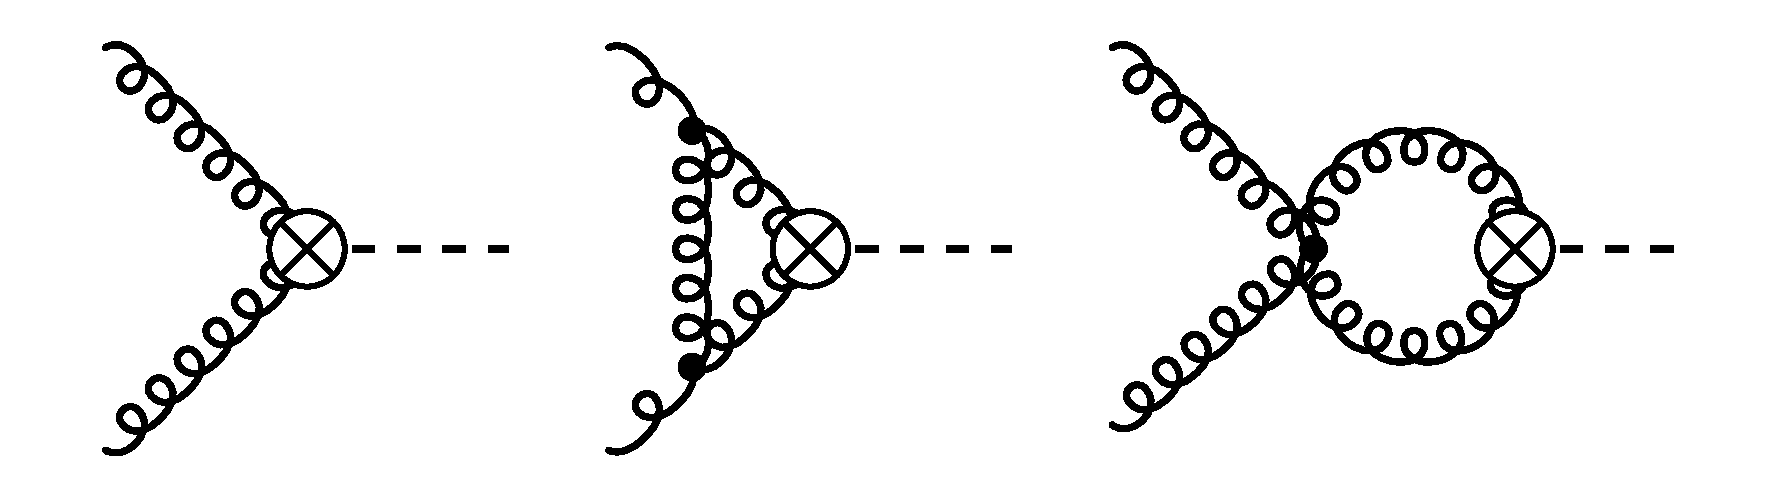
\includegraphics[scale=0.3]{Images/NLO_Feynman_diagrams/ggH.pdf}
\caption{One-loop corrections to the Higgs-gluon form factor. The first diagram contributes through the NLO Wilson coefficient.}
\label{fig:4:ggH}
\end{figure}
Using Eq.~\eqref{eq:4:ggH_cross_section} for the partonic $gg \rightarrow H$ cross section, we then find
\begin{equation}
\begin{split}
&\hat{\sigma}_{gg \rightarrow H} = \frac{\pi}{576 v^2} \xi  \left(\frac{\alphas}{\pi} \right)^2 \delta(1 - \xi) \\
&\qquad \times \left[ \left( 1 + \epsilon + \BigO{\epsilon^2} \right) + \frac{\alphas}{\pi} \left(\frac{m_H^2}{\mu^2} \right)^{-\epsilon} \left(-\frac{3}{\epsilon^2} - \frac{3}{\epsilon} + \frac{5}{2} + \frac{7 \pi^2}{4} + \BigO{\epsilon} \right) + \BigO{\alphas^2} \right]
\end{split}
\end{equation}
where we defined $\xi$ as the of the Higgs mass over the partonic center of mass energy
\begin{equation}
  \xi = \frac{m_H^2}{s} = \frac{m_H^2}{\tau S}.
\end{equation}
\begin{figure}
  \centering
  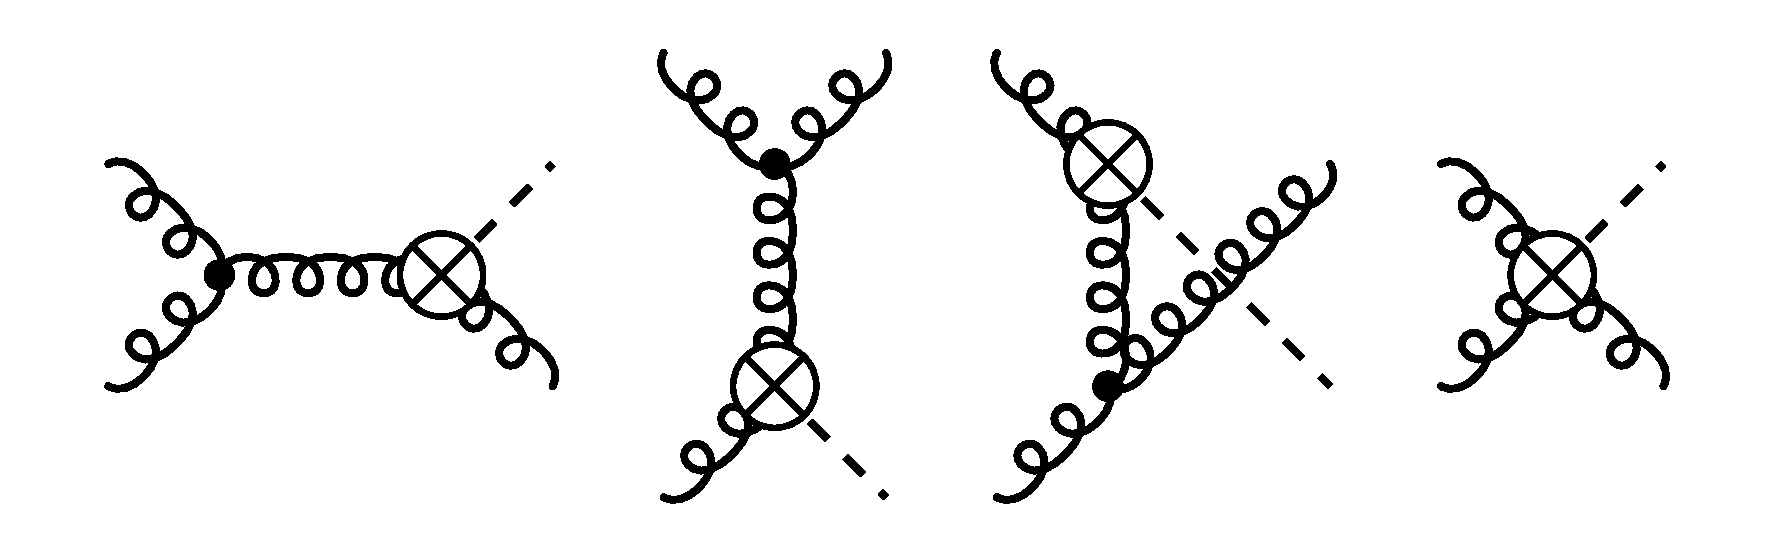
\includegraphics[scale=0.3]{Images/NLO_Feynman_diagrams/ggHg.pdf}
  \caption{Feynman diagrams for the real radiation corrections in the gluon-gluon channel.}
  \label{fig:4:ggHg}
\end{figure}

As expected, the \acs{NLO} partonic cross section is not finite on its own, because the \acs{IR} divergences only cancel in inclusive observables. We must therefore also compute the real radiation corrections as well as the contributions from collinear renormalization. For the former, we evaluate the diagrams in Fig.~\ref{fig:4:ggHg} and obtain the averaged squared amplitude
\begin{equation}
\overline{|\mathcal{M}_{gg \rightarrow H g}|^2} = \frac{1}{N_A^2 4 (1 - \epsilon)^2} \frac{\alphas^3}{v^2} \left(\frac{32}{3 \pi} \right) \left[ (1 - 2 \epsilon) \frac{m_H^8 + s^4 + t^4 + u^4}{stu} + \frac{\epsilon}{2} \frac{\left(m_H^4 + s^2 + t^2 + u^2 \right)^2}{stu} \right],
\label{eq:4:ggHg_Amp}
\end{equation}
where $N_A$ is the dimension of the adjoint representation, \ie\ $N_A = N^2 - 1$ for $\SU{N}$ groups. The symbols $s$, $t$ and $u$ denote the usual \textit{Mandelstam variables}. Since the Mandelstam variables are not completely independent, as they must satisfy
\begin{equation}
  s + t + u = m_H^2,
\end{equation}
the squared matrix element only depends on the final state momenta through $t$ or $u$. The phase-space integral is $2*d$ dimensional. We can reduce one of the $d$ dimensional integrals via the momentum conserving delta function. Using spherical coordinates and the remaining two delta functions which ensure on-shellness of the Higgs and the final state gluon, we can carry out the energy and momentum magnitude integral explicitly. This is particularly simple in the center of mass frame. We are hence left with an integral over the $\mathcal{S}_1^{d - 2}$ sphere. If we now apply the recursion relation
\begin{equation}
\int_{\mathcal{S}_1^{d - 2}} = \int \dd \cos \theta \sin^{d - 4} \theta \int_{\mathcal{S}_1^{d - 3}},
\end{equation}
and use that the amplitude only depends on the azimuthal angle, \ie\ the scattering angle of the Higgs (or gluon), we can carry out the integral over the $\mathcal{S}_1^{d - 3}$ sphere explicitly. In the end the phase-space integral is a single one-dimensional integral
\begin{equation}
\text{P.S.} = \frac{1}{8 \pi} \frac{1}{\Gamma (1 - \epsilon)} \left(\frac{s}{\mu^2 e^{\gamma_E}}\right)^{-\epsilon} \left(1 - \xi \right)^{1 - 2 \epsilon} \Theta (1 - \xi) \int_0^1 \dd \omega \, \omega^{-\epsilon} (1 - \omega)^{-\epsilon},
\end{equation}
where $\omega$ is related to the scattering angle of the Higgs via
\begin{equation}
\omega = \frac{1 + \cos \theta}{2}.
\end{equation}

The amplitude in Eq.~\eqref{eq:4:ggHg_Amp} is proportional to $1/tu$, \ie\ it diverges if the final state gluon becomes collinear to one of the initial state gluons. Consequently, we expect the appearance of poles once we perform the phase-space integration. Indeed, we find after a straightforward integration
\begin{equation}
\begin{split}
& \hat{\sigma}_{gg \rightarrow H g} = \frac{1}{576 \pi^2} \frac{\alphas}{v} \left(1 - \xi \right)^{-1 - 2 \epsilon} \left( \frac{s}{\mu^2} \right)^{-\epsilon} \Theta (1 - \xi) \\
& \quad \times \left[ - \frac{3}{\epsilon} \left(1 + \xi^4 + (1 - \xi)^4 \right) - \frac{11}{2} (1 - \xi)^4 - 6 (1 - \xi + \xi^2)^2 + \epsilon \left( \frac{3 \pi^2}{2} - 6 + (1 - \xi)\cdot \left(\cdots \right) \right) \right].
\label{eq:4:sigma_ggHg}
\end{split}
\end{equation}

The cross section also has a soft singularity at $\xi \rightarrow 1$, which can be regulated by applying the distributional identity in Eq.~\eqref{eq:2:distributional_identity}. The $\BigO{\epsilon}$ terms proportional to $(1 - \xi)$ we only hinted at in Eq.~\eqref{eq:4:sigma_ggHg} will hence not contribute as they are only integrated together with the delta function $\delta (1 - \xi)$. The final result then reads
\begin{equation}
\begin{split}
& \hat{\sigma}_{gg \rightarrow H g} = \frac{1}{576 \pi^2} \frac{\alphas^3}{v^2} \left(\frac{s}{\mu^2} \right)^{-\epsilon} \Theta (1 - \xi) \bigg \lbrace \left[ \frac{3}{\epsilon^2} + \frac{3}{\epsilon} + 3 - \frac{3 \pi^2}{4} \right] \delta(1 - \xi) \\
&\quad - \frac{6 \xi}{\epsilon} \left[ \frac{\xi}{(1 - \xi)_+} + \frac{1 - \xi}{\xi} + \xi (1 - \xi) \right] (1 + \epsilon) - \frac{11}{2} (1 - \xi)^3 \\
& \quad + 6 \left(\frac{\log (1 - \xi)}{1 - \xi} \right)_+ \left[1 + \xi^4 + (1 - \xi)^4 \right]  \bigg \rbrace.
\end{split}
\label{eq:4:sigma_ggHg_full}
\end{equation}

The poles proportional to the delta function $\delta (1 - \xi)$ exactly cancel between real~\eqref{eq:4:sigma_ggHg_full} and virtual contributions~\eqref{eq:4:ggH_cross_section}. The remaining divergences should cancel after coupling and collinear renormalization. According to Eq.~\eqref{eq:2:initialDiv}, the additional contribution from collinear renormalization is
\begin{equation}
\hat{\sigma}_{gg \rightarrow Hg}^C = 2 \times \frac{\alphas}{2 \pi} \frac{1}{\epsilon} \int_0^1 \dd z\, P_{gg}^{(0)}(z) \hat{\sigma}_{gg \rightarrow H} (z s) = \frac{1}{576 \pi^2} \frac{\alphas^3}{v^2} \frac{1}{\epsilon} \xi P_{gg}(\xi) (1 + \epsilon).
\end{equation}
With the definition of the splitting kernel in Eq.~\eqref{eq:2:Altarelli_Parisi_splitting_functions}, we see that the remaining poles in the real radiation contribution are indeed canceled. The additional pole introduced by the collinear renormalization is finally canceled by the charge renormalization. Gathering the fruits of our labor, we determined that the inclusive partonic cross section at \acs{NLO} reads
\begin{equation}
\begin{split}
& \hat{\sigma}_{gg \rightarrow HX} = \frac{\alphas^2}{576 \pi v^2} \Theta(1 - \xi) \bigg \lbrace \delta(1 - \xi) \\
& \quad + \frac{\alphas}{\pi} \bigg [ \delta(1 - \xi) \left(\pi^2 + \frac{11}{2} \right) - \frac{11}{2} \left(1 - \xi \right)^3 + 6 \left( 1 + \xi^4 + (1 - \xi)^4 \right) \left(\frac{\log (1 - \xi)}{1 - \xi} \right)_+ \\
& \hspace{10cm} + \xi P_{gg}(\xi) \log \left(\frac{s}{\mu^2} \right) \bigg ] \bigg \rbrace
\end{split}
\label{eq:4:ggHX_NLO_HTL_cross_section}
\end{equation}

We can carry out the same analysis for the $q \bar{q}$ and $q g$ channel. The Feynman diagrams are depicted in Fig.~\ref{fig:4:qqHg}.
\begin{figure}[h]
\centering
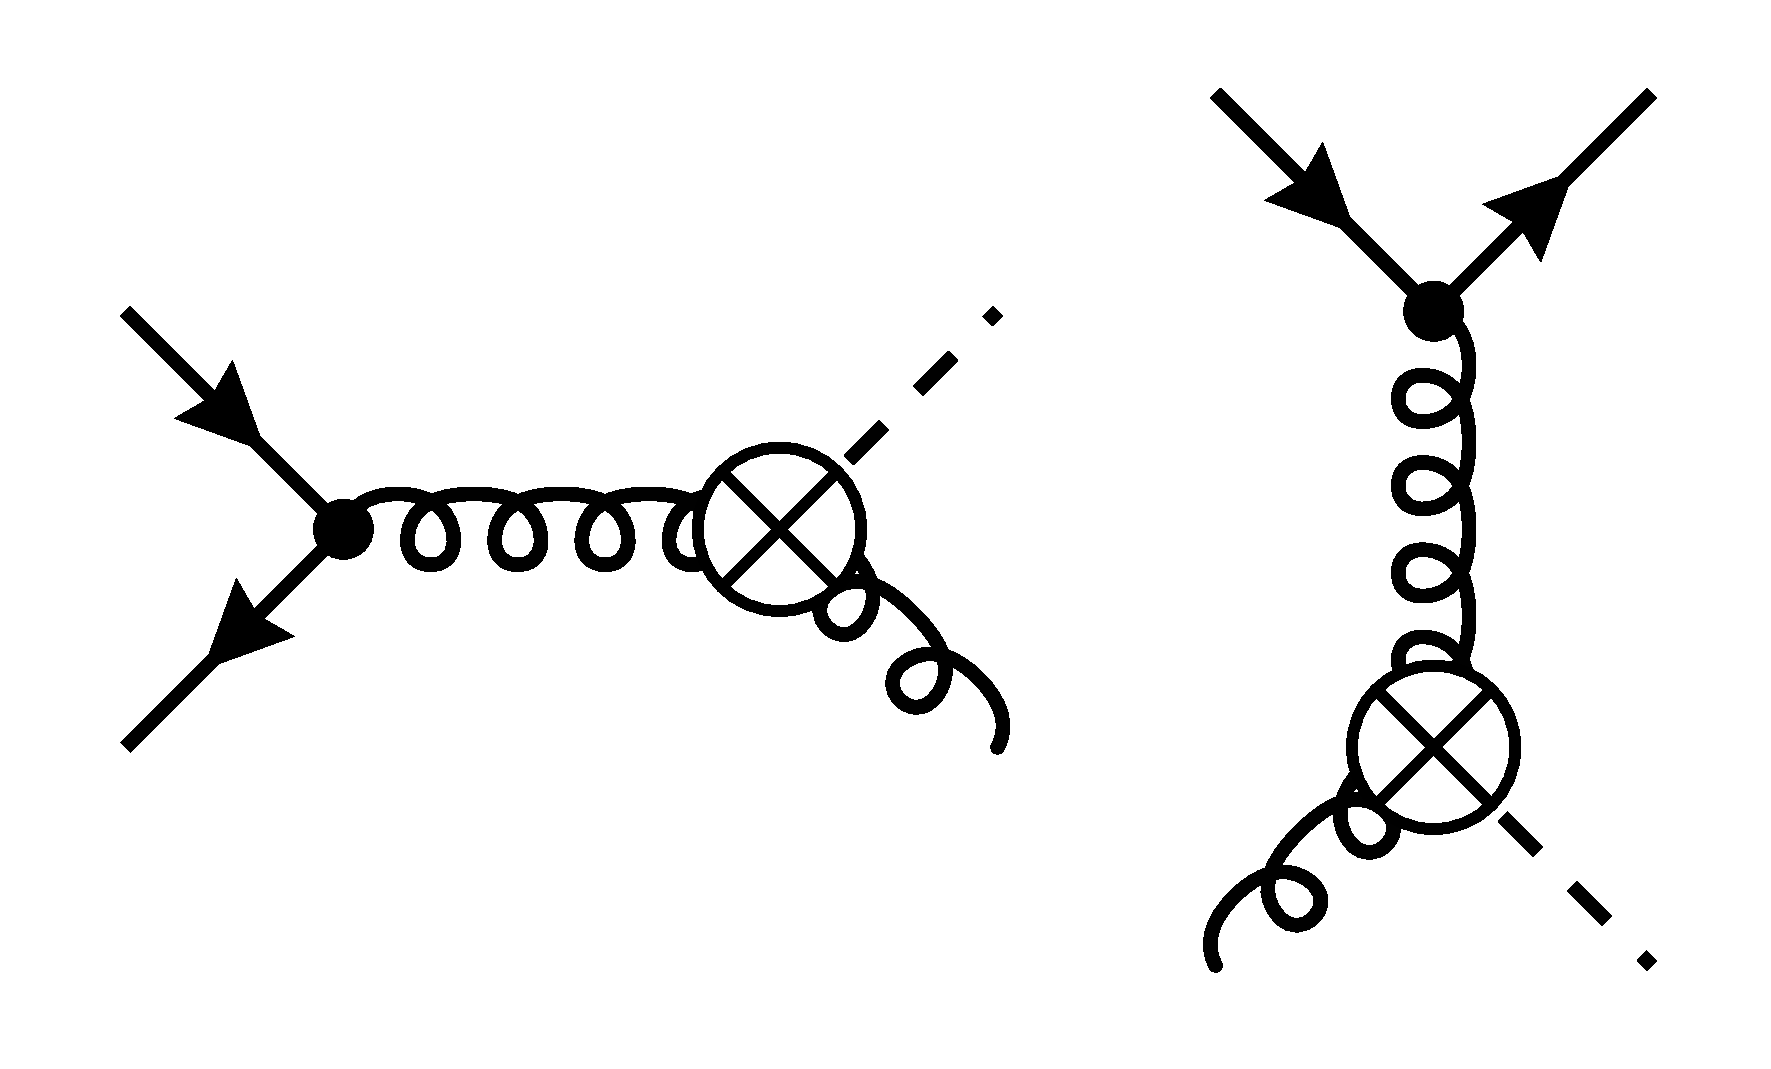
\includegraphics[scale=0.15]{Images/NLO_Feynman_diagrams/qqHg.pdf}
\caption{Feynman diagrams contributing to the $q \bar{q}$ (left) and $q g$ (right) channel of the Higgs production cross section.}
\label{fig:4:qqHg}
\end{figure}
The amplitude for $q \bar{q} \rightarrow H g$ does not exhibit any collinear or soft divergences, rendering collinear renormalization unnecessary. The result for the cross section reads
\begin{equation}
\hat{\sigma}_{q \bar{q} \rightarrow H g} = \frac{1}{486 \pi^2} \frac{\alphas^3}{v^2} \Theta (1 - \xi) \left(1 - \xi \right)^3.
\end{equation}
The $qg$-channel on the other hand has a collinear divergence when the final state quark becomes collinear to the initial state quark. After collinear renormalization we find for the cross section
\begin{equation}
\begin{split}
&\hat{\sigma}_{qg \rightarrow Hg} + \hat{\sigma}_{qg \rightarrow Hg}^C = \frac{\alphas^3}{576 \pi^2 v^2} \Theta (1 - \xi) \\
& \hspace{4cm} \times \bigg \lbrace (1 - \xi) \frac{3 \xi - 7}{3} + \frac{1}{2} \xi P_{gq}(\xi) \left[1 + \log\!\left(\frac{s}{\mu^2} \right) +2 \log\!\left(1 - \xi \right) \right] \bigg \rbrace.
\end{split}
\end{equation}

\begin{figure}[h]
\centering
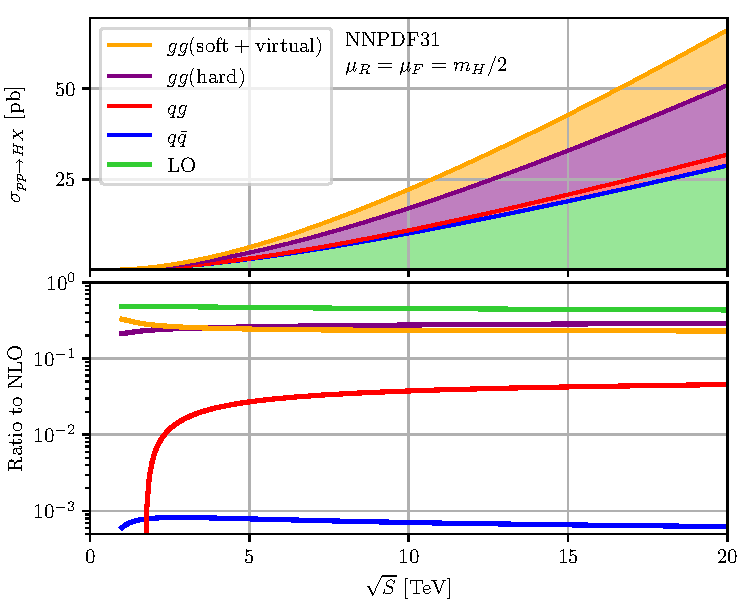
\includegraphics[width=\figurewidth]{Images/channel_comparison_HTL_NLO.pdf}
\caption{Hadronic cross section as function of the hadronic center of mass energy. The total cross section is partinioned into its various channels. The channel denoted ``soft + virtual'' collects the leading terms of the threshold expansion around $(1 - \xi)$ in Eq.~\eqref{eq:4:ggHX_NLO_HTL_cross_section}, that is all terms proportional to $\delta (1 - \xi)$ and irreducible plus distributions. The lower plot shows the ratio of the various channels to the leading order cross section. Computational setup is described in the \hyperref[chap:notation_and_conventions]{conventions}.}
\label{fig:4:channel_comparison}
\end{figure}
After convolution of the partonic cross section with the partonic luminosity we get the hadronic cross section, which is displayed in Fig.~\ref{fig:4:channel_comparison} as a function of the hadronic center of mass energy. The cross section is split into the various channels. The ``soft + virtual'' channel denotes all contributions which originate from integrating the delta function $\delta (1 - \xi)$ and irreducible plus distributions, \ie\ terms of the form
\begin{equation}
a
\end{equation}
At \acs{NLO}, it only comes from gluon-induced Higgs production~\eqref{eq:4:ggH_cross_section}.

The majority of the hadronic cross section is due to a gluon-gluon initial state, making up more than 95\% over the full spectrum of energies. Roughly half of this contribution comes from \acs{LO}. The other half is composed, yet again of roughly two equal parts, the ``soft + virtual'' contribution and the remaining real radiation part. The quark-gluon initial state has the second largest impact, whereas the quark-quark induced Higgs production is completely negligible, contributing below 1\textperthousand. The large suppression of the $q\bar{q}$ channel is almost entirely due to the reduced partonic luminosity of the channel. Indeed, from Fig.~\ref{fig:2:luminosity}, we see that the $q \bar{q}$ flux is roughly 30 times smaller than the $q g$ one. This is also the order of magnitude of the ratio of the $qg$ and $q \bar{q}$ induced Higgs production cross section.

The gluon-gluon and quark-gluon luminosity on the other hand is rather similar, especially close to the production threshold, where most of the contributions to the cross section comes from, since larger values are suppressed by $\mathcal{L}/\tau$. Yet we observe that quark-gluon-channel contribution is almost an order of magnitude smaller than in the gluon-gluon channel. To investigate the origin of this suppression, we can look at the coefficient of the logarithm $\log (\mu^2)$ which is predetermined by the \acs{RGE}
\begin{equation}
\frac{\partial \hat{\sigma}_{qg \rightarrow Hq}}{\partial \log \mu^2} = -\frac{\alphas}{2 \pi} \int_0^1 \dd \xi \, P_{gq}(\xi) \hat{\sigma}_{gg \rightarrow H}, \quad \frac{\partial \hat{\sigma}_{gg \rightarrow Hg}}{\partial \log \mu^2} = -2 \times \frac{\alphas}{2 \pi} \int_0^1 \dd \xi \, P_{gg}(\xi) \hat{\sigma}_{qg \rightarrow H}.  \
\end{equation}
At the threshold, the ratio quark-gluon to gluon-gluon logarithmic coefficients is thus $C_F/(4 C_A) = 1/9$, which is also roughly the ratio we observed in their contribution to the cross section. The origin of the suppression, is thus partly due to the difference in the color factor and the additional combinatorial factors in the gluon-gluon channel.

Since the \acs{NLO} corrections are of the same magnitude as the \acs{LO} cross section, the perturbative result is not yet reliable. One would need to go to even more loops and higher multiplicities in the hope to reach perturbative convergence.

\todo{In the integration with the luminosity, I have to not apply the plus distributions onto the luminosity in order to get consistent results with SusHi. Why is that?}

\subsection{Phenomenological Application}
Having discussed the \acs{HTL} at length, it is important to investigate how well the approximation works for phenomenological applications. In Fig.~\ref{fig:4:HTL_accuracy}, we show the relative error of the cross section in the \acs{HTL} compared to the results with a finite quark mass for different powers of $\alphas$ in the various partonic channels.

\begin{figure}[h]
\centering
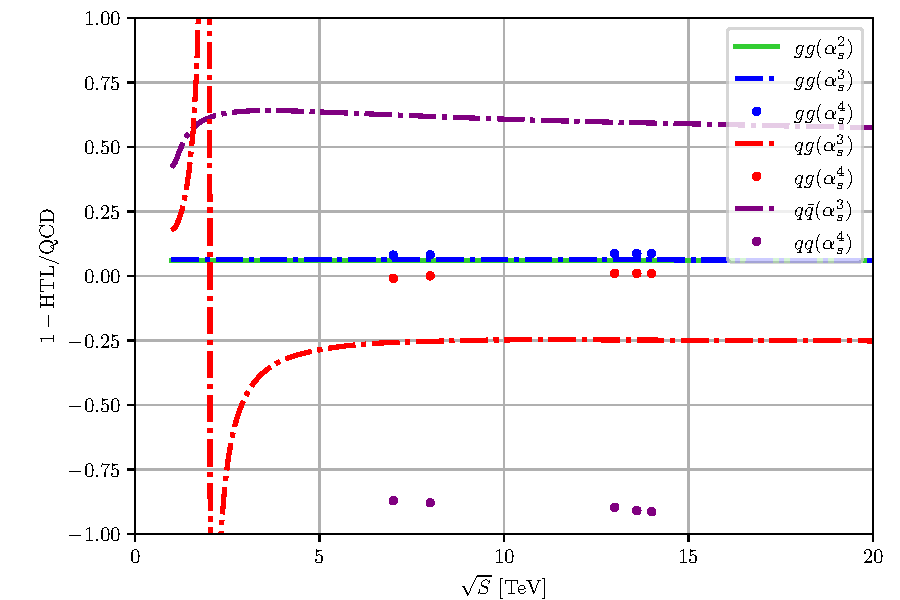
\includegraphics[width=\figurewidth]{Images/HTL_accuracy.pdf}
\caption{Relative error of the \acs{HTL} compared to the results with finite top-quark mass for various center of mass energies. Displayed are contributions to the cross section in each partonic channels. The computational setup is described in the \hyperref[chap:notation_and_conventions]{conventions}. The methods to compute the \acs{NNLO} results with finite top-quark mass are described in chapter \ref{chap:5:computational_details}.}
\label{fig:4:HTL_accuracy}
\end{figure}
At \acs{LO}, the \acs{HTL} underestimates the cross section by around $6.5$\%. In the \acs{HTL}, the Higgs-gluon form factor, is accurate up to power corrections of order $z = m_H^2/4m_t^2 \approx 13\%$, so the observed accuracy of the approximation aligns with our expectations. For radiative corrections, $m_H^2/m_t^2 \approx 52\%$ is the more natural expansion parameter and the quark-gluon as well as the quark-quark channel show, that they are indeed only roughly $50\%$ accurate.

The gluon-gluon channel on the other hand shows a remarkable property: the accuracy of the \acs{HTL} stays quite constant across perturbative orders in $\alphas$. In our opinion, this feed is explained by the fact, that much of the structure of the perturbative corrections is dictated by lower orders, and that, for this channel in particular, these kinds of corrections turn out to be numerically large. Indeed, we can apply \textit{Catani's I operator}~\cite{Catani:1996vz} to predict the poles, as well as the overall factor $(-m_H^2/\mu^2)^{-\epsilon}$, of the Higgs-Gluon form factor in Eq.~\eqref{eq:4:HTL_formfactor}. So the part of the partonic cross section which is derived from \acs{LO} reads
\begin{equation}
  \begin{split}
  &\hat{\sigma}_{gg \rightarrow H} \Big \vert_{\propto \sigma_{gg \rightarrow H}^{(0)}} = \frac{\pi}{576 v^2} \xi  \left(\frac{\alphas}{\pi} \right)^2 \delta(1 - \xi) \\
  &\qquad \times \left[ \left( 1 + \epsilon + \BigO{\epsilon^2} \right) + \frac{\alphas}{\pi} \left(\frac{m_H^2}{\mu^2} \right)^{-\epsilon} \left(-\frac{3}{\epsilon^2} - \frac{3}{\epsilon} - 3 + \frac{3 \pi^2}{2} + \BigO{\epsilon} \right) + \BigO{\alphas^2} \right].
  \end{split}
\end{equation}
Numerically, the finite part is largely dominated by the $\pi^2$ term which we obtained from the analytic continuation of the logarithm. One could say, that the analytic continuation causes a large logarithm.

For the real radiation cross section, we can once again already anticipate initial state collinear as well as the soft divergences
\begin{equation}
  \begin{split}
  & \hat{\sigma}_{gg \rightarrow H g} = \frac{1}{576 \pi^2} \frac{\alphas}{v} \left(1 - \xi \right)^{-1 - 2 \epsilon} \left( \frac{s}{\mu^2} \right)^{-\epsilon} \Theta (1 - \xi) \\
  & \quad \times \left[ - \frac{1}{\epsilon} \xi (1 - \xi) P_{gg}^{(0)}(\xi) \frac{2 (-1 + 2 \epsilon) \Gamma (-\epsilon)}{\Gamma (3 - 2 \epsilon)} +  (1 - \xi)^2 \cdot (\cdots)  \right].
  \end{split}
\end{equation}
The $(1 - \xi)^2$ terms, which we denoted by $(\cdots)$ are finite and regular in the soft limit $\xi \rightarrow 1$. We know, that there cannot be any terms of order $(1 - \xi)$ apart from those in the splitting function, because every term in the matrix element \eqref{eq:4:ggHg_Amp} which is constant in the soft limit, still has collinear divergences in the phase-space. \Ie\ all next to soft contributions are captured in the splitting function. In fact, if we compare with the cross section in Eq.~\eqref{eq:4:sigma_ggHg}, then we see that the actual lowest order term is even $(1 - \xi)^4$.

The partonic luminosity together with the factor $1/\tau$ cause a strong enhancement of the phase-space region close to the threshold $\xi \rightarrow 1$ or $\tau \rightarrow m_H^2/S$. Therefore, the hadronic cross section will be well approximated by convoluting the inclusive cross section
\begin{equation}
\begin{split}
& \hat{\sigma}_{gg \rightarrow HX} \Big \vert_{\propto \sigma_{gg \rightarrow H}^{(0)}} = \frac{\alphas^2}{576 \pi v^2} \Theta(1 - \xi) \bigg \lbrace \delta(1 - \xi) \\
& \quad + \frac{\alphas}{\pi} \bigg [ \delta(1 - \xi) \pi^2\left( \frac{3}{4} + \BigO{1/\pi^2} \right) + 6 \left( 1 + \xi^4 + (1 - \xi)^4 \right) \left(\frac{\log (1 - \xi)}{1 - \xi} \right)_+ \\
& \hspace{10cm} + \xi P_{gg}(\xi) \log \left(\frac{s}{\mu^2} \right) \bigg ] \bigg \rbrace.
\end{split}
\end{equation}

Numerically, we find that the approximation is around $90\%$ accurate at \acs{NLO}. The main deviations are caused by the soft-virtual channel. We can therefore expect to see deviations in the rescaling factor
\begin{equation}
r^{\mathrm{N}^n\mathrm{LO}} = \frac{\sigma_{gg \rightarrow HX}^{\mathrm{QCD}, \mathrm{N}^n \mathrm{LO}}}{\sigma_{gg \rightarrow HX}^{\mathrm{HTL}, \mathrm{N}^n \mathrm{LO}}}
\end{equation}
across perturbative orders of the order of $10\%\times z \approx 1\%$.
\todo{Add reference to results for finite top-quark masses.}

Strictly speaking, our discussion was limited to \acs{NLO}. However, we claim that most of the arguments, especially those concerning the real radiation corrections, are transferable to higher orders in perturbation theory.

We can leverage the small corrections on the rescaling parameter to improve the \acs{HTL} cross section results by rescaling the \acs{HTL} results by
\begin{equation}
\sigma_{gg \rightarrow HX}^{\mathrm{rHTL}, \mathrm{N}^n\mathrm{LO}} = r^{\mathrm{LO}} \sigma_{gg \rightarrow HX}^{\mathrm{HTL}, \mathrm{N}^n\mathrm{LO}},
\end{equation}
where the superscript ``\acs{rHTL}'', now refers to the \textit{rescaled heavy top limit}. Since the gluon-gluon channel is the dominant production channel and the rescaling factor remains quite constant across the perturbative orders, the \acs{rHTL} cross section will yield a good approximation ($\sim 1 \%$) for the Higgs production cross section\footnote{Excluding the effects from light quark masses.}.




\section{Theory Status}
Having analyzed the gluon-gluon fusion Higgs production cross section at \acs{LO}, and \acs{NLO} in the \acs{HTL}. We are now equipped with all concepts to discuss state-of-the-art theory predictions.

As already mentioned, the most precise theoretical predictions come from N${}^3$LO cross sections in the \acs{HTL}~\cite{Anastasiou:2015vya, Anastasiou:2016cez}. They apply the method of reverse unitarity (see section \ref{subsec:phase_space_integration}) to perform the phase-space integration fully analytically. The cross section is calculated in terms of a deep expansion in the threshold parameter $(1 - \xi)$
\begin{equation}
\hat{\sigma}_{ij \rightarrow HX} = \delta_{ig} \delta_{jg} \hat{\sigma}_{\mathrm{SV}} + \sum_{n = 0}^N c_{ij}^{(n)} (1 - \xi)^n,
\end{equation}
where $\hat{\sigma}_{\mathrm{SV}}$ is the leading term, the soft-virtual contribution we already encountered. The soft-virtual contribution has been calculated in Ref.~\cite{Anastasiou:2014vaa}. Because the partonic luminosity is concentrated heavily around the threshold region, one would expect, to see good convergence of the hadronic cross section. Indeed, Ref.~\cite{Anastasiou:2015vya} computed the first 37 terms of the threshold expansion found that the hadronic cross section is already well approximated by the first five terms.

In the meantime, results without reliance on the threshold expansion have become available~\cite{Mistlberger:2018etf}, confirming the expected accuracy of the threshold expansion and shifting the total cross section by around $+0.10\ \mathrm{pb}$ at $13\ \TeV$.

In Fig.~\ref{fig:4:energy_scan_rHTL} we show the results for the gluon-gluon fusion cross section in the \acs{rHTL} at various perturbative orders as a function of the hadronic center of mass energy.
\begin{figure}[h]
\centering
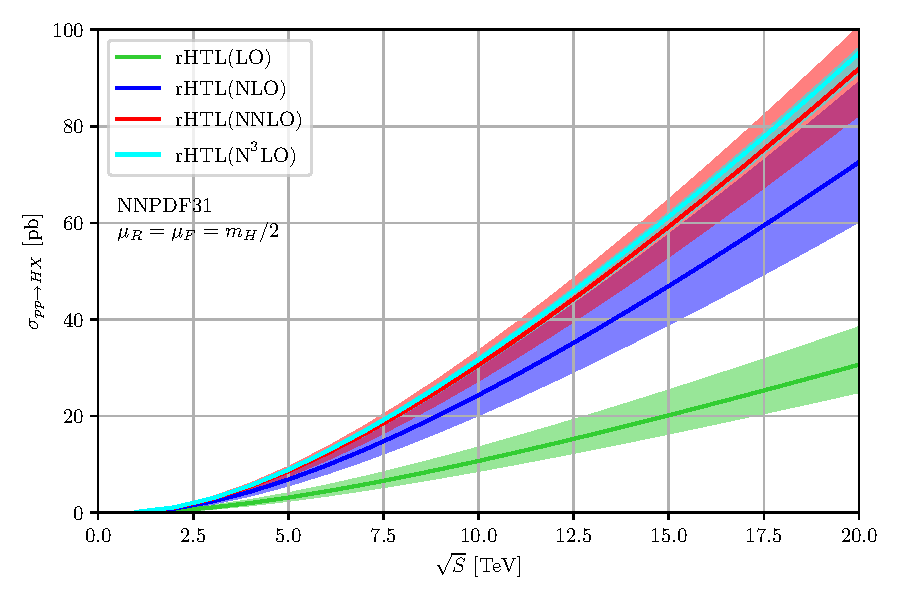
\includegraphics[width=\figurewidth]{Images/energy_scan_HTL.pdf}
\caption{Gluon-gluon fusion hadronic cross section as a function of the center of mass energy. Displayed are results computed in the \acs{rHTL} at various perturbative orders. Transparent bands indicate the scale uncertainty calculated with seven-point scale variation. The computational setup is described in the \hyperref[chap:notation_and_conventions]{conventions}.}
\label{fig:4:energy_scan_rHTL}
\end{figure}

As we discussed before, the \acs{NLO} cross section is about twice as large as predicted in the Born approximation. \acs{NNLO} corrections are still sizeable, contribution roughly $20\%$ to the cross section. The \acs{NLO} scale uncertainties underestimate the effect of higher orders, as the central \acs{NNLO} cross section is outside the previous uncertainty bands. Only when we go to N${}^3$LO do we see perturbative convergence and corrections, consistent with the previous scale uncertainty bands.

\subsection{Scale Uncertainties}
\subsection{PDF-Theory Uncertainties}
\subsection{Electroweak Corrections}
\subsection{Finite Top-Quark Mass Effects}
\subsection{Effect of Light Quarks}
